\section{Introduction}
Over the past decade, there has been significant progress in the development of Advanced Driver Assistance Systems (ADAS) and autonomous driving technologies. ADAS technologies have become increasingly intelligent, and autonomous driving technology is progressing beyond level 2 towards level 3 of driving automation defined by Society for Automotive Engineers (SAE) \cite{sae20213016}. 
% This means that there is a growing amount of time during which the driver is not actively involved in the driving task. 
However, there is not the mass production of technology that has surpassed level 3 of driving automation is still not available, and there are three main reasons as follows: safety, interpretability, and ride comfort.
In level 3, the system must be liable for all potential accidents that occur during its operation. 
Therefore, ensuring safety is of utmost importance. To ensure safety, it is necessary to redundantly acquire various perception information.
Then, claiming responsibility means being able to provide justifications for the system's perception information.
Ensuring interpretability of the perception information is also essential.
In addition to quantitative perception information such as distance to preceding vehicles, relative velocity, and time to collision (TTC), more intuitive information is needed.
Lastly, there is the issue of ride comport. 
One crucial issue that should not be overlooked in the widespread adoption of ADAS and autonomous driving technology is motion sickness \cite{diels2016self, iskander2019car}.
Iskander et al. even used the term an autonomous car sickness \cite{iskander2019car}.
Motion sickness arises from the conflict between sensory inputs, where the detected motion information deviates from the expectation based on past experiences during autonomous driving \cite{reason1975motion,reason1978motion}.
In other words, autonomous driving systems need to drive more like humans.

To mitigate all these challenges, we propose a new method that detects driving vehicle and their brake light status.
The brake light status information is the most fundamental signal for multiple drivers to drive safety on the road.
Humans adjust their driving patterns based not only on distance and relative velocity but also on the brake light status of neighboring vehicles. 
Autonomous driving systems that need to be safer should not overlook this fundamental information.
Moreover, brake light status is particularly intuitive.
While distance, relative velocity, and TTC may be clearer information among machines, brake light status information possesses a much more effective interpretability when communicating with humans.
Furthermore, ADAS that considers the brake light status of preceding vehicles can improve ride comfort \cite{pirhonen2022predictive}.
Therefore, considering the brake light status in ADAS of autonomous driving systems can acquire redundantly interpretable perceptual information, which enhances intuitive understanding.
And it can drive in a more human-like manner, ultimately reducing sensory conflict and alleviating motion sickness.


% There are various theories explaining the causes of motion sickness, but this study focuses specifically on the sensory conflict theory. 
% According to this theory, motion sickness occurs due to a conflict between sensory inputs, where the detected motion information deviates from the expectation based on past experiences \cite{reason1975motion,reason1978motion}. 
% For instance, in the case of adaptive cruise control (ACC), which intelligently follows the preceding vehicle by considering factors such as distance, relative velocity, and time to collision (TTC), many drivers and passengers experience discomfort and motion sickness due to the discrepancy between their previous experiences and the system's actions. 
% One of the main causes of this discrepancy is the system's failure to consider the operation of the preceding vehicle's brakes. Humans adjust their following patterns based not only on the distance and relative velocity but also on the operation of the preceding vehicle's brakes. 

\begin{figure}[]
    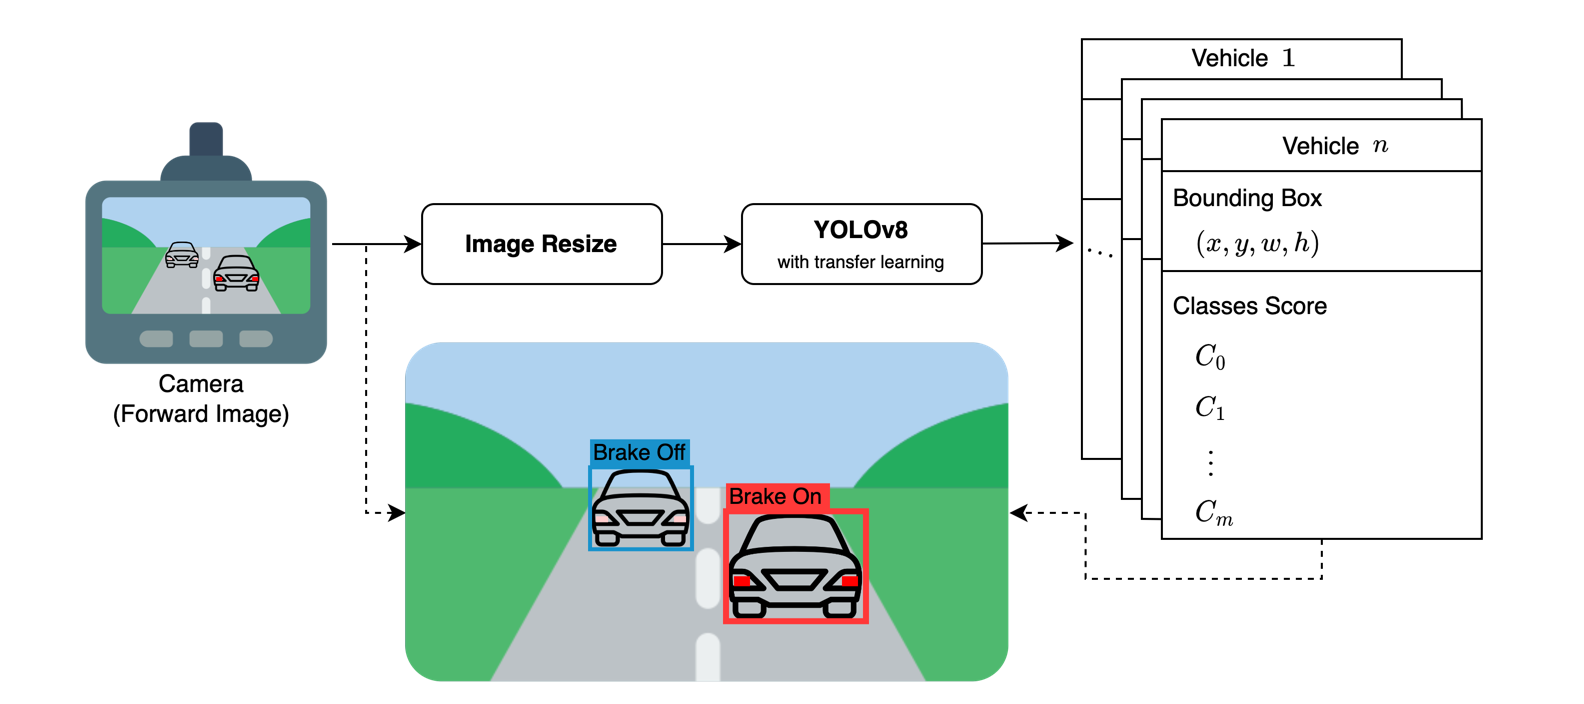
\includegraphics[scale=0.5]{fig/workflow.png}
    \caption{Workflow of the proposed one-stage brake light detection network. The solid line arrows represent the flow of data for inference purposes, while the dashed line arrows represent the flow of data for visualization purposes.}
    \label{fig:workflow}
\end{figure}

In this paper, we propose a one-stage neural network that detects brake lights of preceding vehicles, taking into account the trade-off between inference time and accurate detection performance. 
The proposed network is based on YOLOv8 \cite{YOLOv8}, the latest version of the popular one-stage object detection network, and leverages transfer learning to perform the task of detecting driving vehicles and brake lights as shown in Figure \ref{fig:workflow}.
Existing research on brake light detection utilizing computer vision or artificial neural network techniques exists, but they typically employ multi-stage architectures of two or more stages, neglecting the inference time.

We collected more than 11K real-world driving images and manually annotated the driving vehicle and brake light status for each image for transfer learning with YOLOv8. 
Based on the collected dataset, we conducted transfer learning of YOLOv8 models and evaluated the performance of the models in terms of model size, brake light status, and ambient lighting conditions.
The real-time performance of the trained models was verified using an edge device, Nvidia Jetson Nano, installed in the driving vehicle.
This allowed us to assess the model's ability to make predictions in real-time while considering its computational efficiency.

The main contributions in this study can be described as follows:
\begin{itemize}
    \item We propose a one-stage network for detecting the brake light status of vehicles in the forward image during driving. The proposed network takes a single image as input and outputs bounding boxes for all vehicles present in the image, along with the detection of whether their brake light is on or off. 
    \item We introduce a dataset for the task of driving vehicle and brake light status detection during driving. The dataset consists of over 11K real-world driving images captured under various conditions including day, night, and tunnel. For all the collected image has annotations for vehicle bounding boxes and brake light status, which are manually annotated by experts.
    \item The proposed detection network based on YOLOv8 is fine-tuned using the introduced dataset. The trained model achieve high detection performance and the real-time performance of the model on an edge-device is verified.
\end{itemize}

The rest of this paper is organized as follows. 
Section \ref{sec:related} introduces related works on the general object detection algorithm and brake light status detection. 
Section \ref{sec:proposed} discusses the proposed detection network and dataset for the transfer learning.
Section \ref{sec:experiments} presents the details of transfer learning and analyzes the evaluation results.
Section \ref{sec:conclusions} concludes this work and describes further work. 